\documentclass[12pt,a4paper]{book} % article, report, book.
%%%%%%%%%%%%%%%%%%%%%%%%%%%%%%%%%%%%%%%%%%%%%%%%%%%%%%%%%%%%%%%%%%%
%%% Documento LaTeX                                             %%%
%%%%%%%%%%%%%%%%%%%%%%%%%%%%%%%%%%%%%%%%%%%%%%%%%%%%%%%%%%%%%%%%%%%
% Título: Paquetes
% Autor:  Ignacio Moreno Doblas
% Fecha:  2014-02-01
%%%%%%%%%%%%%%%%%%%%%%%%%%%%%%%%%%%%%%%%%%%%%%%%%%%%%%%%%%%%%%%%%%%
% Tabla de materias:
% 1 Codificación e idioma %
% 2 Matemáticas y Física %
% 3 Gráficos%
% 4 Estilo y formato%
%%%%%%%%%%%%%%%%%%%%%%%%%%%%%%%%%%%%%%%%%%%%%%%%%%%%%%%%%%%%%%%%%%%

%1 Codificación e idioma%
\usepackage[utf8]{inputenc} %Codificación en utf8%
\usepackage[spanish]{babel} %Hyphenation (Guionado) en español%
\usepackage[T1]{fontenc} %Codificación de fuente%
\usepackage{eurofont} %Tipografía euro (€)%

%2 Matemáticas y Física %
% Importante para ecuaciones, magnitudes y unidades%
\usepackage{amssymb,amsmath,latexsym,amsfonts} % paquetes estándar%
\usepackage[squaren]{SIunits} %Paquete para magnitudes y unidades físicas%
\usepackage{ifthen} %sentencias if y while%

%3 Gráficos%
\usepackage{graphics,graphicx} %paquetes gráficos estándar%
\usepackage{wrapfig} %paquete para gráfica lateral%
\usepackage[rflt]{floatflt} %figuras flotantes%
  % \begin{floatingfigure}[r]/[l]{4.5cm}
  % \end{floatingfigure}
\usepackage{graphpap} %comando \graphpaper en el entorno picture%

%4 Estilo y formato%
\usepackage{fancyhdr} %cabeceras y pies mejor que con \pagestyle{}%
\usepackage{titlesec,titletoc} %Formateo de secciones y títulos%
\raggedbottom %Para fragmentar versos en varias páginas%
\usepackage{makeidx} %MakeIndex%
%\usepackage{showidx} % Hace que cada comando \index se imprima en la página donde se ha puesto (útil para corregir los índices)
\usepackage{alltt} % Define el environment alltt, como verbatim, excepto que \, { y } tienen su significado normal. Se describe en el fichero alltt.dtx.
\usepackage[pdftex,bookmarksnumbered,hidelinks]{hyperref} %hyper-references%
\usepackage{minitoc} % Para poner tablas de contenido en cada capítulo.
\usepackage{listings} % Para escribir piezas de código C, Python, etc. %
%listings configuration
\lstset{
  language=[ARM]Assembler, %Puede ser C, C++, Java, etc.
  showstringspaces=false,
  formfeed=\newpage,
  tabsize=4,
  commentstyle=\itshape,
  basicstyle=\ttfamily,
  morekeywords={models, lambda, forms}
}

\usepackage{tipa} % tipografía IPA (International Phonetic Alphabet)
\usepackage{longtable} %Entorno Longtable, fracciona tablas a lo largo de páginas%
\usepackage{colortbl}
\usepackage{acronym}  %Para expandir automáticamente los acrónimos

%%%%%%%%%%%%%%%%%%%%%%%%%%%%%%%%%%%%%%%%%%%%%%%%%%%%%%%%%%%%%%%%%%%
% Tabla de materias:
% 1 Información del Documento %
% 2 Comandos a nivel de texto %
% 3 Comandos a nivel de entorno %
% 4 Comandos a nivel de página y sección %
% 5 Otros comandos %
%%%%%%%%%%%%%%%%%%%%%%%%%%%%%%%%%%%%%%%%%%%%%%%%%%%%%%%%%%%%%%%%%%%

% 1 Información del Documento %
\newcommand{\pfctitlename}{Guiones de prácticas sobre la plataforma Raspberry Pi}
\newcommand{\pfcauthorname}{Antonio José Villena Godoy}
\newcommand{\pfctutorname}{Rafael Asenjo Plaza \\ Francisco Javier Corbera Peña}
\newcommand{\pfcanno}{2015}

% 2 Comandos a nivel de texto %
\newcommand{\R}{\textsuperscript{\textregistered}}  %Símbolo registrado%
\newcommand{\C}{\textsuperscript{\copyright}} %Símbolo Copyright%
\newcommand{\TM}{\texttrademark} %Símbolo Trade Mark (marca comercial)%

% 2.1 Comandos abreviatura %
\newcommand{\tit}{\textit} %Fuente cursiva (itálica)%
\newcommand{\tbf}{\textbf} %Fuente negrita%
\newcommand{\ttw}[1]{\texttt{#1}} %Fuente máquina de escribir (typewriter)%
%Combinación%
\newcommand{\textittt}[1]{\textit{\texttt{#1}}} %itálica y typewriter%
\newcommand{\textittw}{\textittt} % Otra forma de escribirlo.
\newcommand{\tittw}{\textittw} %Shortened%
\newcommand{\tbftw}[1]{\tbf{\ttw{#1}}}

%Crea una nueva línea y la indenta sin crear interlineado extra.
\newcommand{\nli}{\\ \indent} 

%Para escribir un correo electrónico%
\newcommand{\mailto}[1]{\href{mailto:#1}{#1}}

% Si vas a hacer un uso básico de \index (entradas en el índice de sólo un nivel, sin formatos especiales, etc.), define la orden
\newcommand{\miindex}[1]{#1\index{#1}}

\newcommand{\hs}{\hspace} % Abreviatura espacio horizontal
\newcommand{\vs}{\vspace} % Abreviatura espacio vertical

% Abreviaturas para los conjuntos de números más comunes.
\newcommand{\realnumbers}{\mathbb R}
\newcommand{\naturalnumbers}{\mathbb N}
\newcommand{\integernumbers}{\mathbb Z}
\newcommand{\rationalnumbers}{\mathbb Q}
\newcommand{\complexnumbers}{\mathbb R}
\newcommand{\irrationalnumbers}{\mathbb I}

% Doble barra sobre una letra (para expresar las matrices).
\newcommand{\doublebar}[1]{\bar{\bar{#1}}} 
% Ej: \vector(y) = \doublebar(A) \vector(x) (Stma. lineal de ec.)

% 3 Comandos a nivel de entorno %
\newcommand{\benu}{\begin{enu}} % Begin enumerate
\newcommand{\eenu}{\end{enu}}   % End enumeration

%Comando para escribir código Python
\newcommand{\code}[3]{
  %\hrulefill
  %\subsection*{#1}
  %\subsubsection{#1}
  \lstinputlisting{#2}
  %#1\\
  \begin{table}[h!]
    \centering
    \caption{#1}
    \label{#3}
  \end{table}
  \vspace{2em}
}

% 4 Comandos a nivel de página y sección %
%Crea página en blanco
\newcommand{\blankpage}{\clearpage{\pagestyle{empty}\cleardoublepage}}

% Versión x del comando section: sin numeración pero sí aparece en la tabla de contenidos.
\newcommand{\sectionx}[1]{
  \section*{#1}
  \addcontentsline{toc}{section}{#1}
}

% Versión y del comando section: sin numeración y NO aparece en la tabla de contenidos.
\newcommand{\sectiony}[1]{
  \section*{#1}
}

% Versión x del comando chapter: sin numeración pero sí  aparece en la tabla de contenidos.
\newcommand{\chapterx}[1]{
  \chapter*{#1}
  %\addcontentsline{toc}{chapter}{#1} %Caused by minitoc package%
  \addstarredchapter{#1} %For minitoc package%
}

% substituto del comando \chapter: incluye estilo de página.
\newcommand{\chapterbegin}[1]%
  {%
    \pagestyle{fancy}
    \fancyhead[LE,RO]{\thepage}
    \fancyhead[LO]{Capítulo \thechapter. #1}
    %\fancyhead[RE]{Parte \thepart \rightmark} %
    \fancyhead[RE]{\nouppercase{\rightmark}} %
        
    \chapter{#1}
  }

% Versión x del comando \chapterbegin: sin numeración y aparece en la tabla de contenidos.
\newcommand{\chapterbeginx}[1]%
  {%
    \pagestyle{fancy}
    \fancyhead[RO,LE]{\thepage}
    \fancyhead[RE,LO]{#1}
    %\fancyhead[LO]{Chapter \thechapter}
    %\fancyhead[RE]{Part \thepart} %
    
    \chapterx{#1}
  }

%Fin de capítulo
\newcommand{\chapterend}{\pagestyle{empty}\cleardoublepage \thispagestyle{empty}}
%Si fuera un artículo en lugar un libro, \clearpage en lugar de \cleardoublepage

% 5 Otros comandos %
%\let\Oldpart\part
%\newcommand{\parttitle}{}
%\renewcommand{part}[1]{\Oldpart{#1}\renewcommand{\parttitle}{#1}} %Header customization%

%Cambiar el título índice de capítulo a ``Contenido''.
\renewcommand{\mtctitle}{Contenido}

\dominitoc % Para tablas de contenidos por capítulo.

\addto{\captionsspanish}{
  \renewcommand{\listtablename}{Índice de Tablas}
  \renewcommand{\tablename}{Tabla} } % Por ejemplo, modificar el nombre de 'Cuadro' a 'Tabla'.

\addto{\captionsspanish}{
  \renewcommand{\contentsname}{Índice} }

%Si se desea cambiar el tipo de letra a Arial
% por cualquier razón, descomentar las siguientes
% dos líneas
%\renewcommand{\rmdefault}{phv} % Arial
%\renewcommand{\sfdefault}{phv} % Arial
  
%\addto{\captionsspanish}{
% \renewcommand{\partname}{Fase} }

%\addto{\captionsspanish}{%
%    \renewcommand{\refname}{\vspace{-4.5ex}}} % Para que no aparezca el texto 'referencias' en la bibliografía.

% Modifica el interlineado
%\renewcommand{\baselinestretch}{1.5}

   \definecolor{myfboxbg}{gray}{0.9}
   \newsavebox{\efcaja}
   \newenvironment{myfbox}{\begin{lrbox}{\efcaja}}
               {\end{lrbox}{\colorbox{myfboxbg}{\usebox{\efcaja}}}}

%%%%%%%%%%%%%%%%%%%%%%%%%%%%%%%%%%%%%%%%%%%%%%%%%%%%%%%%%%%%%%%%%%%
% Tabla de materias:
%--------------------%
% 1 dobleindent
% 2 izqindent
% 3 dobleindentx
% 4 ite
% 5 descript
% 6 enu
% 7 itemization
% 8 sinopsis
% 9 objetivo
%%%%%%%%%%%%%%%%%%%%%%%
% Para conocer los parámetros de diseño de las listas, tales como
%  los márgenes izquierdo, derechos y los diferentes saltos,
%  véase el archivo ``List layout.png'' que acompaña esta plantilla.
% Así se conocerá mejor cómo adaptar un entorno según los requisitos 
%  del usuario.

%%%%%%%%%%%%%%%%%%%%%%%
% Definición de longitudes para usar en los entornos:
%
% Normal parskip.
\newlength{\parskipenv}
\setlength{\parskipenv}{\parskip}

\newlength{\parindentenv}
\setlength{\parindentenv}{\parindent}
%%%%%%%%%%%%%%%%%%%%%%%

% 1 dobleindent
%El entorno dobleindent está pensando para escribir párrafos con doble indentación a cada lado.
%Tiene dos parámetros de entrada con las distancias medidas desde los márgenes de página.

\newenvironment{dobleindent}[2]
  %Comienzo de nuevo entorno%
  {
  \begin{list}
    {}
    {
    % Left and right margins:
    \leftmargin = #1 
    \rightmargin = #2
    %
    % Separation from preceding and following text:
    \topsep = 0ex
    \partopsep = 0ex
    \parsep = \parskipenv
    %
    % Indentation for paragraphs:
    \itemsep = \parskipenv
    \itemindent = \parindentenv
    \listparindent = \itemindent
    %
    % Horizontal separation from label:
    \labelsep = 1ex
    \settowidth{\labelwidth}{0cm}
    }
    
     \item}
  % End new env
  {\end{list}}

%%%%%%%%%%%%%%%%%%%%%%%%%%%%%
%2 izqindent
% El entorno izqindent sólo crea un párrafo indentado a la izquierda.
\newenvironment{izqindent}[1]
{
\begin{dobleindent}{#1}{0cm}
}
{
\end{dobleindent}
}

%%%%%%%%%%%%%%%%%%%%%%%%%%%%%
% 3 dobleindentx
% El entorno dobleindentx es una variación del dobleindent usando leftskip y rightskip.
% Aunque es más limitado, también se puede usar.
\newenvironment{dobleindentx}[2] % Sólo funciona en modo paragraph
{ % Preamble
  \leftskip = #1
  \rightskip = #2
}
{ % Postamble
\leftskip = 0cm
\rightskip = 0cm
}

%%%%%%%%%%%%%%%%%%%%%%%%%%%%%
% 4 ite
% El entorno ite es una modificación del entorno itemize estándar de \LaTeX. Puede usarse o modificarse si el usuario lo desea.
% También puede parametrizarse el entorno enumerate o description de forma equivalente.
\newenvironment{ite}
  {
    \begin{izqindent}{\parindent}
    \hspace{-\parindent}  % compensación del sangrado que introduce el entorno.
    \vspace{-1.0\parskip} % compensación del \parskip que introduce el entorno.
    \vspace{-\baselineskip} % compensación por la línea que introduce el entorno.
    \begin{itemize}
  }
  {
    \end{itemize}
    \end{izqindent}
  }

%%%%%%%%%%%%%%%%%%%%%5
% commando stdformat para formatear los entornos descript, enu y itemization.
\newcommand{\stdformat}
  {% Declarations for format presentation.
    %     
    % Separation from preceding and following text:
    \setlength{\topsep}{0ex}%
    \setlength{\partopsep}{0ex} %
    %
    % Horizontal separation from label:
    \labelsep = 1ex
    \setlength{\labelwidth}{0ex}
    %
    % Left and right margins: 
    \setlength{\leftmargin}{1cm}%
    \addtolength{\leftmargin}{\labelsep}
    \setlength{\rightmargin}{0ex}
    %  
    % Indentation for paragraphs:
    \setlength{\itemindent}{-\leftmargin}%
    \addtolength{\itemindent}{1ex}
    \setlength{\listparindent}{\parindent}%
    %   
    % Separation between paragraphs.
    \setlength{\parsep}{\parskipenv}% 
    \setlength{\itemsep}{1ex}
  }

%%%%%%%%%%%%%%%%%%%%%%%%%%%%%
% 5 descript

\newenvironment{descript}
  % Beginning new env def.
  {
    \begin{list}
      {} % No default label for \item.
      {
        % Declarations for format presentation.
        \stdformat
        %
        \renewcommand{\makelabel}[1]{\normalfont\bfseries##1\hfil}
      }
  }
  % Ending new env def.
  {
    \hspace*{\fill} \\ \end{list}
  } % Se introduce un salto de línea para que el texto siguiente esté separado.
%END newenvironment{descript}

%%%%%%%%%%%%%%%%%%%%%%%%%%%%%
% 6 enu
\newcounter{itemnumber} % Counter for the environment.

\newenvironment{enu}
  % Beginning new env def.
  {
    \begin{list}
    {
      \raggedleft \arabic{itemnumber}
    }
    {
      \usecounter{itemnumber}
      \stdformat
    }
  }
  {
    \end{list}
  }

%%%%%%%%%%%%%%%%%%%%%%%%%%%%%
% 7 itemization
\newenvironment{itemization}
  % Beginning new env def.
  {
    \begin{list}
      {$\bullet$} % No default label for \item.
      {
        % Declarations for format presentation.
        \stdformat
      }
  }
  % Ending new env def.
  {
    \end{list}
  }


%%%%%%%%%%%%%%%%%%%%%%%%%%%%%
% 8 sinopsis
\newenvironment{sinopsis}{%[1]{
  \sectiony{Sinopsis}
  %\label{#1}
} {
  \pagebreak
}

%%%%%%%%%%%%%%%%%%%%%%%%%%%%%
% 9 objetivo
\newenvironment{objetivo}{%[1]{
  \sectiony{Objetivo}
  %\label{#1}
} {
}

%%%%%%%%%%%%%%%%%%%%%%%%%%%%%%%%%%%%%%%%%%%%%%%%%%%%%%%%%%%%%%%%%%%
% Tabla de materias:
%--------------------%
% 1 Márgenes de página
%%%%%%%%%%%%%%%%%%%%%%%
% Para conocer los parámetros de diseño de páginas, tales como
%  los márgenes izquierdo, derecho, anchura de página, etc.
%  véase el archivo ``Page layout.png'' que acompaña esta plantilla.
% Así se conocerá mejor cómo adaptar el documento según los 
%  requisitos del usuario.

% 1 Márgenes de página
%-------------------------------%
% Parámetros de estilo de página.
% DIN A4: 29.7 cm x 21 cm
%   área neta: 3 cm + 3 cm + 15 cm.
%
% Definición de márgenes de página
%  even para páginas pares
%  odd  para páginas impares
\newlength{\realoddsidemargin}    % \oddsidemargin menos 1 in.
\newlength{\realevensidemargin}   % \evensidemargin menos 1 in.
\newlength{\realtopmargin}        % \topmargin menos 1 in.
%
% Asignación de márgenes de página
% ASIGNESE en caso de querer cambiarlo
\setlength{\realtopmargin}{2cm}     % REAL top margin.
\setlength{\realoddsidemargin}{3cm}   % REAL oddside margin.
\setlength{\realevensidemargin}{3cm}  % REAL evenside margin.
\setlength{\hoffset}{0cm}
\setlength{\voffset}{0cm}
%
% Substracción de 1 pulgada de compensación
%  (véase ``Page Layout.png'' para más información)
\addtolength{\realoddsidemargin}{-1in}  % 1 inch = 2.54 cm.
\addtolength{\realevensidemargin}{-1in}
\addtolength{\realtopmargin}{-1in}
%
% Asignación de anchuras y márgenes
% No hay notas al margen
\setlength{\marginparsep}{0cm} % No van a existir notas al margen
\setlength{\marginparwidth}{0cm} % No van a existir notas al margen
%
% Asignación de anchura de texto
\setlength{\textwidth}{15cm}  % Anchura neta del texto (globalmente).
%
% Asignación de márgenes par, impar y en altura
\setlength{\oddsidemargin}{\realoddsidemargin}  % odd-page left margin (global).
\setlength{\evensidemargin}{\realoddsidemargin} % even-page left margin (global).
\setlength{\topmargin}{\realtopmargin}          % top margin (Global).

% Se puede usar también el paquete chngpage.

%%%%%%%%%%%%%%%%%%%%%%%%%%%%%%%%%%%%%%%%%%%%%%%%%%%%%%%%%%%%%%%%%%
%   1 Length commands.          %
%-------------------------------%
% Defines new length command (e.g., \newlength{\gnat}}
% \newlength{}
%
% Set lenght to a value.
% \setlength{\gnat}{length}
% \addtolength{}{}
%
% Sets the value of a length command equal to the width of a specified piece of text; e.g., \settowidth{\parindent}{\em small}.
% \settowidth{}{}
% Set the value of a height. e.g., \settoheight{\parskip}{Gnu}
% \settoheight{}{}
% Set the value that extends below the line. e.g., \settodepth{\parskip}{gnu}.
% \settodepth{}{}
%
% To multiply a length, write: 7.0\gnat = \gnat * 7.0
%%%%%%%%%%%%%%%%%%%%%%%%%%%%%%%%%%%%%%%%%%%%%%%%%%%%%%%%%%%%%%%%%%

\begin{document}

%%%%%%%%%%%%%%%%%%%%%%%%%%%%%%%%%%%%%%%%%%%%%%%%%%%%%%%%%%%%%%

\chapterbegin{Tipos de datos y sentencias de alto nivel}
\label{chp:TipDat}
\minitoc

{\bf Objetivo}:
En esta sesión repasaremos cómo se representa la
información en la memoria del computador: veremos la definición en
ensamblador de punteros, vectores y matrices. También veremos cómo se programan las
estructuras de alto nivel del tipo {\tt if-else} y los bucles {\tt
for} y {\tt while}.

\section{Lectura previa}

\subsection{Modos de direccionamiento del ARM}

En la arquitectura ARM los accesos a memoria se hacen mediante instrucciones
específicas {\tt ldr} y {\tt str} (luego veremos las variantes {\tt ldm},
{\tt stm} y las preprocesadas {\tt push} y {\tt pop}). El resto de instrucciones
toman operandos desde registros o valores inmediatos, sin excepciones. En este
caso la arquitectura nos fuerza a que trabajemos de un modo determinado: primero
cargamos los registros desde memoria, luego procesamos el valor de estos registros
con el amplio abanico de instrucciones del ARM, para finalmente volcar los
resultados desde registros a memoria. Existen otras arquitecturas como la Intel x86,
donde las instrucciones de procesado nos permiten leer o escribir directamente
de memoria. Ningún método es mejor que otro, todo es cuestión de diseño. Normalmente
se opta por direccionamiento a memoria en instrucciones de procesado en arquitecturas
con un número reducido de registros, donde se emplea la memoria como almacén
temporal. En nuestro caso disponemos de suficientes registros, por lo que podemos
hacer el procesamiento sin necesidad de interactuar con la memoria, lo que por otro
lado también es más rápido.

\begin{descript}
  \item[Direccionamiento inmediato.]
    El operando fuente es una constante, formando parte de la instrucción.
\begin{lstlisting}
    mov     r0, #1
    add     r2, r3, #4
\end{lstlisting}
  \item[Direccionamiento inmediato con desplazamiento o rotación.]
    Es una variante del anterior en la cual se permiten operaciones intermedias
    sobre los registros.
\begin{lstlisting}
    mov     r1, r2, LSL #1      /* r1 <- (r2*2) */
    mov     r1, r2, LSL #2      /* r1 <- (r2*4) */
    mov     r1, r3, ASR #3      /* r1 <- (r3/8) */
\end{lstlisting}
    Implicitamente también interviene en la creación de constantes, rotando o
    desplazando constantes más pequeñas de forma transparente al usuario. Como todas
    las instrucciones ocupan 32 bits, es técnicamente imposible que podamos cargar
    en un registro cualquier constante de 32 bits con la instrucción {\tt mov}. Por
    esta razón cuando se necesita cargar una constante más compleja en un registro
    (como una dirección a una variable de memoria) no podemos hacerlo con la instrucción
    {\tt mov}, tenemos que recurrir a {\tt ldr} con direccionamiento a memoria. En algunos
    casos es difícil determinar si el ensamblador conseguirá codificar una constante
    por medio de esta técnica, con lo que la única solución es probar.
\begin{lstlisting}
    mov     r1, #0x80000020
\end{lstlisting}
    Ensamblamos y vemos que no da problemas. Sin embargo con esta otra.
\begin{lstlisting}
    mov     r1, #0x80000040
\end{lstlisting}
    El ensamblador nos muestra el siguiente error.
\begin{lstlisting}
intro1.s: Assembler messages:
intro1.s:10: Error: invalid constant (80000040) after fixup
\end{lstlisting}

  \item[Direccionamiento a memoria, sin actualizar registro puntero.]
    Es la forma más sencilla y admite 4 variantes. Después del acceso
    a memoria ningún registro implicado en el cálculo de la dirección
    se modifica.
\begin{itemize}
  \item{\tt [Rx, \#+inmediato] \newline
            [Rx, \#-inmediato] \newline}
    Simplemente añade (o sustrae) un valor inmediato al registro dado
    para calcular la dirección. Es muy útil para acceder a elementos
    fijos de un array, ya que el desplazamiento es constante. Por
    ejemplo si tenemos {\tt r1} apuntando a un array de enteros de
    32 bits {\tt int a[]} y queremos poner a 1 el
    elemento {\tt a[3]}, lo hacemos así.

\begin{lstlisting}
    mov     r2, #1          /* r2 <- 1          */
    str     r2, [r1, #+12]  /* *(r1 + 12) <- r2 */
\end{lstlisting}

    Nótese que hemos multiplicado por 4 el desplazamiento porque cada
    elemento del array son 4 bytes. El desplazamiento no puede ser mayor
    de 12 bits, por lo que nuestro rango está límitado entre {\tt [Rx, \#-4095]}
    y {\tt [Rx, \#+4095]}.

  \item{\tt [Rx, +Ry] \newline
            [Rx, -Ry] \newline}

    Parecido al anterior pero en lugar de un inmediato emplea otro registro. Útil
    en el caso de queramos mantener fijo el registro {\tt Rx} y movernos con {\tt Ry},
    o bien para acceder a desplazamientos mayores a 4095. El mismo ejemplo de
    arriba utilizando esta variante sería.

\begin{lstlisting}
    mov     r2, #1          /* r2 <- 1          */
    mov     r3, #12         /* r3 <- 12         */
    str     r2, [r1, +r3]   /* *(r1 + r3) <- r2 */
\end{lstlisting}

  \item{\tt [Rx, +Ry, operación\_desp \#inmediato] \newline
            [Rx, -Ry, operación\_desp \#inmediato] \newline}

    En este caso aplicamos una operación de desplazamiento
    o rotación sobre el segundo registro {\tt Ry}. Muy útil
    en caso de arrays o estructuras con elementos de longitud
    potencia de 2, ya que podemos indexar directamente. El
    mismo ejemplo de antes.
    
\begin{lstlisting}
    mov     r2, #1
    mov     r3, #3
    str     r2, [r1, +r3, LSL #2]
\end{lstlisting}

    Nótese cómo accedemos a {\tt a[3]}
    directamente con el valor del índice, {\tt 3}).
\end{itemize}


  \item[Direccionamiento a memoria, actualizando registro puntero.]
    En este modo de direccionamiento, el registro que genera la dirección
    se actualiza con la propia dirección. De esta forma podemos recorrer
    un array con un sólo registro sin necesidad de hacer el incremento del
    puntero en una instrucción aparte. Hay dos métodos de actualizar dicho
    registro, antes de ejecutar la instrucción (preindexado) o después
    de la misma (postindexado). Los tres siguientes tipos son los
    postindexados.

\begin{itemize}
  \item{\tt [Rx], \#+inmediato \newline
            [Rx], \#-inmediato \newline}
    Una notación muy parecida a la versión que no actualiza registro, la única
    diferencia es que la constante de desplazamiento queda fuera de los corchetes.
    Presenta el mismo límite de hasta 4095. Este ejemplo pone a cero los 3 primeros
    elementos {\tt a[0], a[1], a[2]} del array.

\begin{lstlisting}
    mov     r2, #0          /* r2 <- 0      */
    str     r2, [r1], #+4   /* a[0] <- r2   */
    str     r2, [r1], #+4   /* a[1] <- r2   */
    str     r2, [r1], #+4   /* a[2] <- r2   */
\end{lstlisting}

  \item{\tt [Rx], +Ry \newline
            [Rx], -Ry \newline}
    Igual que antes pero con registro en lugar de inmediato.

  \item{\tt [Rx], +Ry, operación\_desp \#inmediato \newline
            [Rx], -Ry, operación\_desp \#inmediato \newline}

    Nótese que en todos los modos postindexados
    encerramos entre llaves el primer registro, que es el que se va
    a utilizar en la instrucción de lectura o escritura en memoria. Es decir
    primero cargamos de {\tt [Rx]} y luego actualizamos {\tt Rx} con el valor
    que corresponda. Esta instrucción.

\begin{lstlisting}
    ldr     r2, [r1], +r3, LSL #2
\end{lstlisting}

    Se puede desglosar en estas otras dos, cuyo comportamiento es exactamente
    el mismo.

\begin{lstlisting}
    ldr     r2, [r1]
    add     r1, r1, r3, LSL #2
\end{lstlisting}
\end{itemize}

    Ya hemos visto la notación postindexada. Veamos ahora los tres modos
    preindexados.

\begin{itemize}
  \item{\tt [Rx, \#+inmediato]! \newline
            [Rx, \#-inmediato]! \newline}
    La idea en todos los casos es encerrar entre corchetes la dirección que
    se va a usar en la instrucción. Para diferenciarlo del caso que no actualiza
    el registro le añadimos un {\tt !} al final.

    Este modo es muy útil en casos que queramos reusar en una futura instrucción
    la dirección que hemos calculado. En este ejemplo duplicamos el valor
    que se encuentra en {\tt a[3]}.

\begin{lstlisting}
    ldr     r2, [r1, #+12]!
    add     r2, r2, r2
    str     r2, [r1]
\end{lstlisting}

  \item{\tt [Rx, +Ry]! \newline
            [Rx, -Ry]! \newline}

    Similar al anterior pero usando {\tt Ry} en lugar de inmediato.

  \item{\tt [Rx, +Ry, operación\_desp \#inmediato]! \newline
            [Rx, -Ry, operación\_desp \#inmediato]! \newline}

    Tercer y último caso de direccionamiento preindexado. Al igual que
    antes, desgloso en dos instrucciones para ver el funcionamiento exacto.

\begin{lstlisting}
    ldr     r2, [r1, +r3, LSL #2]!
\end{lstlisting}

    Equivale a esto.

\begin{lstlisting}
    ldr     r2, [r1, +r3, LSL #2]
    add     r1, r1, r3, LSL #2
\end{lstlisting}

    O bien a esto otro.

\begin{lstlisting}
    add     r1, r1, r3, LSL #2
    ldr     r2, [r1]
\end{lstlisting}
\end{itemize}


\subsection{Tipos de datos}

\vspace{0.25cm}
{\bf Tipos de datos básicos.} En la siguiente tabla se recogen los diferentes tipos de datos básicos
 que podrán aparecer en los ejemplos, así como su tamaño y  rango de
representación.

\vspace{1cm}
\begin{center}
%\begin{table}[h!]
\begin{tabular}{|l|l|c|c|}\hline
 ARM & Tipo en C & bits & Rango \\ \hline
 {\tt .byte}  & {\tt unsigned char} & 8 & 0 a 255 \\
              & ({\tt signed}) {\tt char} & 8 & -128 a 127 \\ \hline
 {\tt .hword} & {\tt unsigned short int} & 16 &  0 a 65.535 \\
 {\tt .short} & ({\tt signed}) {\tt short int} & 16 & -32.768 a 32767 \\ \hline
 {\tt .word}  & {\tt unsigned int} & 32 & 0 a 65.535 \\
 {\tt .int}   & ({\tt signed}) {\tt int} &  32 & -32.768 a 32.767 \\
              & {\tt unsigned long int}  & 32 & 0 a 4294967296 \\ 
              & ({\tt signed}) {\tt long int} &  32 & -2147483648 a 2147483647 \\ \hline
 {\tt .quad}  & {\tt unsigned long long} & 64 &  0 a $2^{64}$ \\
              & ({\tt signed}) {\tt long long} & 64 & -$2^{63}$ a $2^{63}$-1 \\ \hline
\end{tabular}
%\end{table}
\end{center}

Nótese como en ensamblador los tipos son neutrales al signo, lo importante
es la longitud en bits del tipo. La mayoría de las instrucciones (salvo
multiplicación) hacen la misma operación tanto si se trata de un número
natural como si es entero en complemento a dos. Nosotros decidiremos el tipo
mediante las constantes que pongamos o según los flags que interpretemos del
resultado de la operación.
\end{descript}


\noindent{\bf Punteros.} Un {\bf puntero} siempre ocupa 32 bits y contiene
una dirección de memoria. En ensamblador no tienen tanta utilidad como en C,
ya que disponemos de registros de sobra y es más costoso acceder a
las variables a través de los punteros que directamente. En este ejemplo
acceder a la dirección de var1 nos cuesta 2 {\tt ldrs} a través del puntero,
mientras que directamente se puede hacer con uno sólo.


\begin{lstlisting}
.data
var1:           .word   3
puntero_var1:   .word   var1

.text
.global main
main:   ldr     r0, =puntero_var1
        ldr     r1, [r0]
        ldr     r2, [r1]
        ldr     r3, =var1
        bx      lr
\end{lstlisting}

Observamos cómo el valor de {\tt r3} es el mismo que el de {\tt r1}.

\begin{lstlisting}
(gdb) ni 4
0x000083a0 in main ()
(gdb) i r r0 r1 r2 r3
r0             0x1054c  66892
r1             0x10548  66888
r2             0x3      3
r3             0x10548  66888
\end{lstlisting}

Incluso en tipos que en C están basados en punteros como las cadenas,
en ensamblador no es necesario tenerlos almacenados en memoria puesto
que podemos obtener dicho valor en un registro con una única instrucción {\tt ldr}.

\vspace{0.25cm}
\noindent{\bf Vectores.} Todos los elementos de un vector se almacenan en un único
bloque de memoria a partir de una dirección determinada. Los
diferentes elementos se almacenan en posiciones consecutivas, de
manera que el elemento {\tt i}  está entre los {\tt i-1} e {\tt i+1}
(figura \ref{fig:dos_3}). Los
vectores están definidos siempre a partir de la posición 0. El propio
índice indica cuántos elementos hemos de desplazarnos respecto del
comienzo del primer elemento (para acceder al elemento cero hemos de
saltarnos 0 elementos, para acceder al elemento 1 hemos de saltarnos
un elemento, etc... En general, para acceder al elemento con índice
{\tt i}
hemos de saltarnos los {\tt i} elementos anteriores).

Dado un vector {\tt int v[N];}, todos los elementos se encuentran en posiciones
consecutivas a partir de la dirección de {\tt v[0]}
(puesto que son {\tt int}, en este ejemplo, cada elemento ocupa 4 bytes). Por lo tanto,
el acceso al elemento {\tt v[i]} se consigue aplicando la siguiente expresión.

\begin{equation}
v[i] = M_d[@v[0] + i*4] 
\label{eq:uno}
\end{equation}

Con $ @v[0]$ nos referimos a la dirección en memoria del elemento
 $ v[0]$. Con $ M_d[\ ]$ notamos el acceso a memoria para la lectura/escritura
de un dato (el número de bytes de memoria implicado dependerá del tipo
de datos declarado). Cuando nos queramos refererir al acceso a memoria
para la obtención de un puntero, lo notaremos como
$ M_{ref}[\ ]$.

\begin{figure}[h]
  \centering
    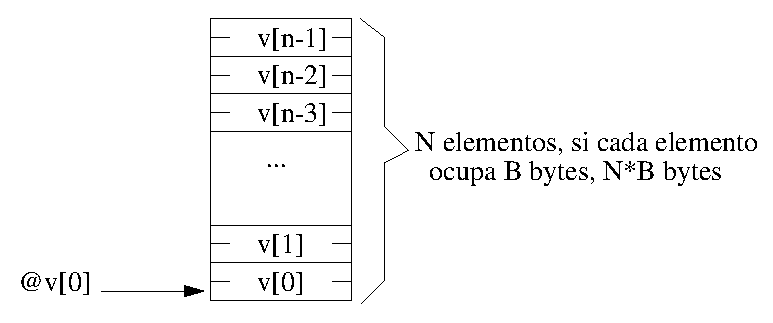
\includegraphics[width=10cm]{graphs/2-3.eps}
  \caption{Representación de un vector en memoria}
  \label{fig:dos_3}
\end{figure}


\noindent{\bf Matrices bidimensionales.} Una matriz bidimensional de N$\times$M
elementos se almacena en un único bloque de memoria. Interpretaremos
una matriz de N$\times$M como una matriz con $N$ filas de $M$ elementos cada
una. Si cada elemento de la matriz ocupa $B$ bytes, la matriz ocupará un
bloque de  $M \times N \times B$ bytes (ver figura \ref{fig:dos_5}(a)).

Dentro de este bloque, los elementos se almacenan por filas. Primero
se guardan todos los elementos de la fila $0$, después todos los de la
fila $1$, etc... Dentro de cada fila, los elementos están ordenados por
columnas (figura \ref{fig:dos_5}(b)).


\begin{figure}[h]
  \centering
    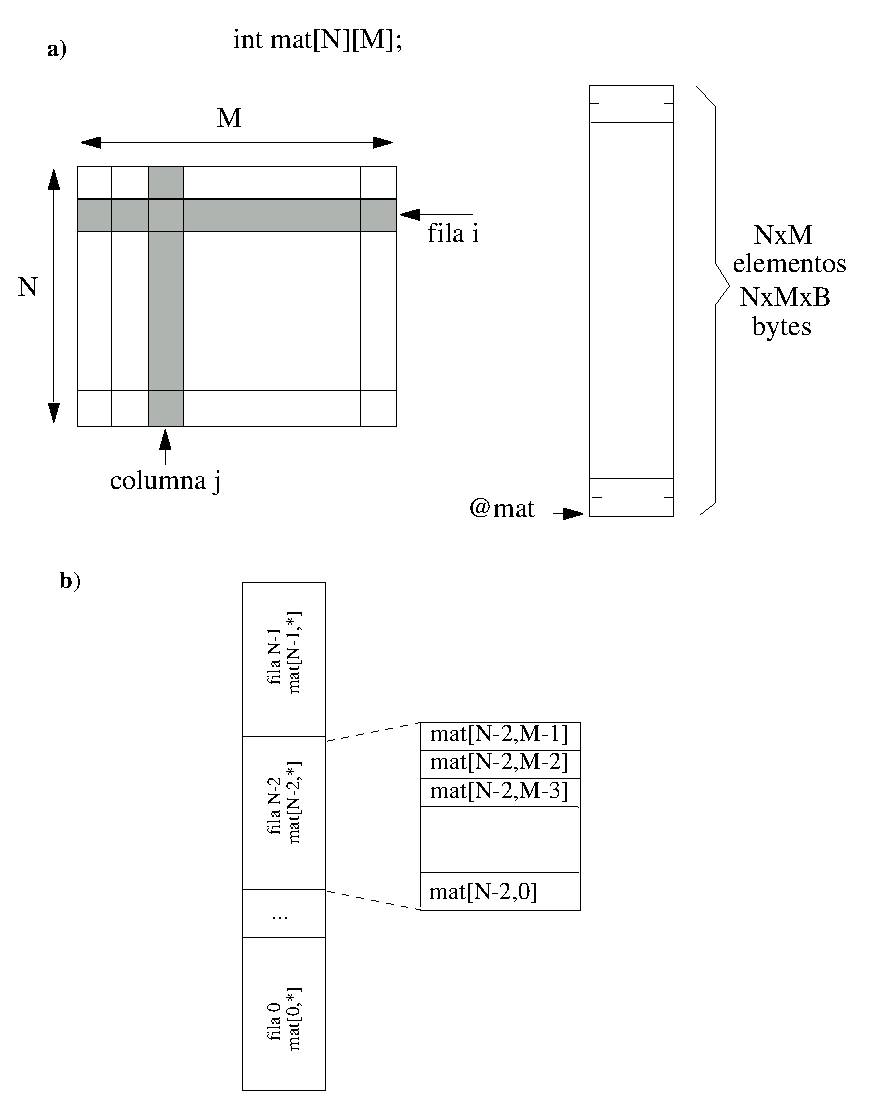
\includegraphics[width=10cm]{graphs/2-5.eps}
  \caption{(a) Formato de una matriz  C con $N$ filas y $M$ columnas y (b)
organización por filas}
  \label{fig:dos_5}
\end{figure}

Por lo tanto, para acceder al elemento {\tt mat[i][j]} hemos de saltar
$i$ filas completas (de $M$ elementos de $B$ bytes) y después $j$
elementos de $B$ bytes (suponiendo una matriz de enteros, $B= 4$ bytes). Es
decir, la fórmula para obtener el elemento {\tt mat[i][j]} será:
\begin{equation}
mat[i][j] = M_d[@mat + ((i*M)+j)*B] 
\label{eq:accesoelemmatriz}
\end{equation}


\subsection{Instrucciones de salto}

Las instrucciones de salto pueden producir saltos incondicionales ({\tt b} y {\tt bx})
o saltos condicionales. En los saltos condicionales añadimos dos o tres letras
a la ({\tt b/bx}), mediante las cuales condicionamos si se salta o no dependiendo
del estado de los flags. Estas condiciones se pueden añadir a cualquier
otra instrucción, aunque la mayoría de las veces lo que nos interesa es controlar
el flujo del programa y así ejecutar o no un grupo de instrucciones dependiendo
del resultado de una operación (reflejado en los flags).

La lista completa de condiciones es ésta.

\begin{itemize}
  \item{\tt EQ} ({\tt eq}ual, igual). Cuando {\tt Z} está activo ({\tt Z} vale 1).
  \item{\tt NEQ} ({\tt n}ot {\tt eq}ual, igual). Cuando {\tt Z} está inactivo ({\tt Z} vale 0).
  \item{\tt MI} ({\tt mi}nus, negativo). Cuando {\tt N} está activo ({\tt N} vale 1).
  \item{\tt PL} ({\tt pl}us, positivo o cero). Cuando {\tt N} está inactivo ({\tt N} vale 0).
  \item{\tt CS/HS} ({\tt c}arry {\tt s}et/{\tt h}igher or {\tt s}ame, carry activo/mayor o igual). Cuando {\tt C} está activo ({\tt C} vale 1).
  \item{\tt CC/LO} ({\tt c}arry {\tt c}lear/{\tt l}ower, carry inactivo/menor). Cuando {\tt C} está inactivo ({\tt C} vale 0).
  \item{\tt VS} (o{\tt v}erlow {\tt s}et, desbordamiento activo). Cuando {\tt V} está activo ({\tt V} vale 1).
  \item{\tt VC} (o{\tt v}erlow {\tt c}lear, desbordamiento inactivo). Cuando {\tt V} está inactivo ({\tt V} vale 0).
  \item{\tt GT} ({\tt g}reater {\tt t}han, mayor en complemento a dos). Cuando {\tt Z} está inactivo y {\tt N=V}({\tt Z} vale 0, {\tt N} vale {\tt V}).
  \item{\tt LT} ({\tt l}ower {\tt t}han, menor en complemento a dos). Cuando {\tt N!=V} ({\tt N} vale {\tt not V}).
  \item{\tt GE} ({\tt g}reater or {\tt e}qual, mayor o igual en complemento a dos). Cuando {\tt N=V}({\tt N} vale {\tt V}).
  \item{\tt LE} ({\tt l}ower or {\tt e}qual, menor o igual en complemento a dos). Cuando {\tt Z} está activo y {\tt N!=V} ({\tt Z} vale 1, {\tt N} vale {\tt not V}).
  \item{\tt HI} ({\tt h}igher, mayor). Cuando {\tt C} está activo y {\tt Z} inactivo ({\tt C} vale 1, {\tt Z} vale 0).
  \item{\tt LS} ({\tt l}ower or {\tt s}ame, menor o igual). Cuando {\tt C} está inactivo ó {\tt Z} activo ({\tt C} vale 0 ó {\tt Z} vale 1).
\end{itemize}

Por ejemplo, la instrucción {\tt beq destino\_salto} producirá un salto
a la instrucción indicada por la etiqueta {\tt destino\_salto} si y sólo
si el bit de estado cero está activo (Z=1), y en caso contrario
(Z=0) no interrumpirá el flujo secuencial de instrucciones.
Previo a un salto condicional, el registro de flags debe ser actualizado
mediante alguna instrucción aritmética ({\tt adds}, {\tt subs}, {\tt cmp},
\dots) o lógica ({\tt and}, {\tt orr}, {\tt tst}, \dots). En la mayoría
de los casos tenemos que añadir el sufijo {\tt s} a una instrucción normal
{\tt add}, para forzar que la nueva instrucción {\tt adds} actualice los flags.

El operando de la instrucción de salto ({\tt b}) puede ser una etiqueta que indica la
posición de memoria a saltar, o bien un registro en caso de {\tt bx}.

Un aspecto muy peculiar de la arquitectura ARM es que las llamadas a
subrutinas se hacen mediante un sencillo añadido a la instrucción de salto. La
instrucción {\tt bl} (también {\tt blx}) hace una llamada a una subrutina,
mediante un salto a la subrutina y escribiendo en el registro {\tt lr} la
dirección de la siguiente instrucción.

\begin{lstlisting}
main:   mov     r1, #1
        mov     r2, #2
        bl      subrut
        mov     r4, #4  /* siguiente instrucción */
        ...

subrut: mov     r3, #3
        bx      lr
\end{lstlisting}

Si seguimos el flujo del programa primero cargamos {\tt r1} a 1, luego {\tt r2}
a 2 y lo siguiente que hay es una llamada a subrutina. En dicha llamada el
procesador carga en {\tt lr} la dirección de la siguiente instrucción {\tt mov r4, \#4}
y salta a la etiqueta {\tt subrut:}. Se ejecuta el {\tt mov r3, \#3} de la subrutina
y después {\tt bx lx} que vendría a ser la instrucción de retorno. Es decir, salimos
de la subrutina retomando el flujo del programa principal, ejecutando {\tt mov r4, \#4}.

Este sencillo esquema vale para un sólo nivel de subrutinas, es decir, dentro de
{\tt subrut} no podemos llamar a otra subrutina porque sobreescribimos el valor del
registro {\tt lr}. La solución para extender a cualquier número de niveles es almacenar
el registro {\tt lr} en pila con las instrucciones {\tt push} y {\tt pop}.

\begin{lstlisting}
main:   mov     r1, #1
        mov     r2, #2
        bl      nivel1
        mov     r5, #5  /* siguiente instrucción */
        ...

nivel1: push    {lr}
        mov     r3, #3
        bl      nivel2
        pop     {lr}
        bx      lr

nivel2: mov     r4, #4
        bx      lr
\end{lstlisting}

Como véis en el último nivel ({\tt nivel2}) podemos ahorrarnos el tener que
almacenar y recuperar {\tt lr} en la pila.

\vspace{0.25cm}
Las instrucciones de salto en la arquitectura ARM abarcan una zona muy extensa,
hasta 16Mb. Sin embargo no cubren todo el ancho del bus de direcciones, sólo
24 de los 32 bits. En caso de necesitar un salto mayor de 24 bits recurrimos
a la misma solución de la carga de inmediatos del {\tt mov}, solo que el
registro a cargar es el {\tt pc}.

\begin{lstlisting}
        ldr pc, =etiqueta
\end{lstlisting}

\subsection{Estructuras de control de alto nivel}

En este punto veremos cómo se traducen a ensamblador las estructuras
de control de alto nivel que definen un bucle ({\tt for}, {\tt while},
\dots), así como las condicionales ({\tt if-else}).

Las estructuras {\tt for} y {\tt while} se pueden ejecutar un mínimo de 0
iteraciones (si la primera vez no se cumple la condición). La traducción de
las estructuras {\tt for} y {\tt while} se puede ver en los listados
\ref{lst:codigoPract2_1} y \ref{lst:codigoPract2_2}.

Para programar en ensamblador estas estructuras se utilizan instrucciones
de salto condicional. Previo a la instrucción de salto es necesario evaluar
la condición del bucle o de la sentencia {\tt if}, mediante instrucciones
aritméticas o lógicas, con el fin de actualizar los flags de estado. La
traducción de la estructura {\tt if} está en los listados
\ref{lst:codigoPract2_3} y \ref{lst:codigoPract2_4}.

\begin{lstlisting}[caption={Código del programa tipos1.c},label={lst:codigoPract2_1},escapeinside={@}{@}]
  int vi, vf, i;

  for ( i= vi; i<=vf; i++ ){ 
    /*cuerpo del bucle*/
  }

  i= vi; 
  while ( i<=vf ){ 
    /*cuerpo del bucle*/
    i++; 
  }
\end{lstlisting}

\begin{lstlisting}[caption={Traducción de las estructuras {\tt for} y {\tt while}.
Hemos supuesto que el valor inicial está en la variable {\tt vi}
y el valor final en  la variable {\tt vf} y se ha utilizado el
registro {\tt r1} como índice de las iteraciones {\tt i}.},label={lst:codigoPract2_2},escapeinside={@}{@}]
        ldr     r1, =vi
        ldr     r1, [r1]
        ldr     r2, =vf
        ldr     r2, [r2]
bucle:  cmp     r1, r2
        bhi     salir
        /* cuerpo
           del
           bucle  */
        add     r1, r1, #1
        b       bucle
salir:
\end{lstlisting}

\begin{lstlisting}[caption={Código del programa tipos2.c},label={lst:codigoPract2_3},escapeinside={@}{@}]
  int a, b;

  if( a==b ){ 
    /* código entonces */
  }
  else{
    /* código sino */
  }
\end{lstlisting}

\begin{lstlisting}[caption={Traducción de la estructura {\tt if}},label={lst:codigoPract2_4},escapeinside={@}{@}]
        ldr     r1, =a
        ldr     r1, [r1]
        ldr     r2, =b
        ldr     r2, [r2]
        cmp     r1, r2
        bne     sino
entonces:
        /* código entonces */
        b       final
sino:
        /* código sino */
final:  ...
\end{lstlisting}

\subsection{Compilación a ensamblador}

Para acabar la teoría veamos cómo trabaja un compilador de C real. Normalmente
los compiladores crean código compilado (archivos {\bf .o}) en un
único paso. En el caso de {\bf gcc} este proceso se hace en dos fases: en una
primera se pasa de C a ensamblador, y en una segunda de ensambladador a código
compilado (código máquina). Lo interesante es que podemos interrumpir justo
después de la compilación y ver con un editor el aspecto que tiene el código
ensamblador generado a partir del código fuente en C.

Veámoslo con un ejemplo.

\begin{lstlisting}[caption={Código del programa tipos3.c},label={lst:codigoPract2_5},escapeinside={@}{@}]
#include <stdio.h>

void main(void){

  int i;

  for ( i= 0; i<5; i++ ){
    printf("%d\n", i);
  }

}
\end{lstlisting}

Después de crear el fichero {\tt tipos3.s}, lo compilamos con este comando.

\begin{lstlisting}
        gcc -Os -S -o tipos3a.s tipos3.c
\end{lstlisting}

Con el parámetro {\tt -S} forzamos la interrupción (generamos {\tt .s} en lugar de
{\tt .o}) y con {\tt -Os} le indicamos al compilador que queremos optimizar en
tamaño, es decir que queremos código ensamblador lo más pequeño posible, sin
importar el rendimiento del mismo.

El código ensamblador resultante está un poco sucio, lleno de directivas superfluas,
con punteros a variables e instrucciones no simplificadas por el preprocesador. Tras
limpiarlo quedaría así.

\begin{lstlisting}[caption={Código del programa tipos3a.s},label={lst:codigoPract2_6},escapeinside={@}{@}]
.data
var1:   .asciz  "%d\012"

.text
.global main
main:   push    {r4, lr}
        mov     r4, #0
.L2:    mov     r1, r4
        ldr     r0, =var1
        add     r4, r4, #1
        bl      printf
        cmp     r4, #5
        bne     .L2
        pop     {r4, pc}
\end{lstlisting}

El carácter {\tt \textbackslash n} se ha transformado en octal {\tt \textbackslash 012} puesto que el ensamblador
no entiende de secuencias de escape. La instrucciones {\tt push} y {\tt pop} son la versión
simple de {\tt stmfd} y {\tt ldmfd} que veremos más adelante. Nótese que la función no acaba
con el típico {\tt bx lr}, se trata de una optimización que consigue reducir de dos
instrucciones a una.

\begin{lstlisting}
        pop     {r4, pc}
\end{lstlisting}

La instrucción anterior es equivalente a estas otras dos.

\begin{lstlisting}
        pop     {r4, lr}
        bx      lr
\end{lstlisting}

En general no vamos a emplear este tipo de optimizaciones en las prácticas, puesto que
dificultan la legibilidad del código.

El resto del código es sencillo de seguir. El registro {\tt r4} hace la función del
contador {\tt i} del bucle, y la salida por pantalla se produce mediante una llamada
a la función printf {\tt bl printf}. Los parámetros se los pasamos a printf mediante
{\tt r0} y {\tt r1} y son un puntero a la cadena a imprimir {\tt \%d\textbackslash n}
y el entero que le vamos a pasar. El porqué se usan estos registros para pasar
parámetros (y el hecho de
haber almacenado {\tt r4} en pila) responde a la convención {\bf AAPCS} que
veremos con más detenimiento en el siguiente capítulo.

Veamos qué ocurre cuando le indicamos al compilador que queremos optimizar al
máximo en velocidad (la escala va del 0 al 3) el mismo código en C.

\begin{lstlisting}
        gcc -O3 -S -o tipos3b.s tipos3.c
\end{lstlisting}

Tras simplificar, el fichero en ensamblador generado sería este.

\begin{lstlisting}[caption={Código del programa tipos3b.s},label={lst:codigoPract2_7},escapeinside={@}{@}]
.data
var1:   .asciz  "%d\012"

.text
.global main
main:   push    {r4, lr}
        mov     r1, #0
        ldr     r4, =var1
        mov     r0, r4
        bl      printf
        mov     r0, r4
        mov     r1, #1
        bl      printf
        mov     r0, r4
        mov     r1, #2
        bl      printf
        mov     r0, r4
        mov     r1, #3
        bl      printf
        mov     r0, r4
        mov     r1, #4
        pop     {r4, lr}
        b       printf
\end{lstlisting}

Observamos que el bucle como tal ha desaparecido. En realidad lo que ha ocurrido
es que el compilador a empleado una técnica agresiva de optimización llamada
{\it loop unrolling} o desenrollamiento de bucle, que consiste en sustituir
mediante repeticiones del cuerpo del bucle, de tal forma que no perdemos tiempo
comparando ni haciendo el salto condicional. En este caso empleamos tantas repeticiones
como iteraciones tiene el bucle, aunque normalmente se llega hasta un límite de
repeticiones. De no ser así el ejecutable se volvería excesivamente grande.

Por último señalar que se optimizado el final de la función, aunque de otra forma
distinta al caso anterior. La última iteración debería ser así.

\begin{lstlisting}
        mov     r0, r4
        mov     r1, #4
        bl      printf
        pop     {r4, lr}
        bx      lr
\end{lstlisting}

\subsection{Ejercicios propuestos.}

\subsubsection{Ejercicio 2.1}
Basándonos en los ejemplos anteriores, escribe un bucle for {\tt for} que imprima
los 50 primeros números pares naturales en orden inverso (desde 100 hasta 2 en pasos
de 2). Una vez hecho esto, aplica desenrollamiento de bucle de tal forma
que el salto condicional se ejecute 10 veces, con 5 repeticiones cada vez.

\begin{center}
\begin{myfbox}
\small
\begin{minipage}{0.92\linewidth}
\begin{center}
\colorbox[gray]{1}{\rule{0cm}{4.5cm}\rule{11cm}{0cm}}
\end{center}
\end{minipage}
\end{myfbox}
\end{center}

\subsubsection{Ejercicio 2.2}
Escribe el código ensamblador correspondiente a una estructura {\tt
if} en la que no exista la rama de {\tt else}.

\begin{center}
\begin{myfbox}
\small
\begin{minipage}{0.92\linewidth}
\begin{center}
\colorbox[gray]{1}{\rule{0cm}{4.5cm}\rule{11cm}{0cm}}
\end{center}
\end{minipage}
\end{myfbox}
\end{center}

\subsubsection{Ejercicio 2.3}

Escribe en ensamblador un código equivalente a éste. Primero
haciendo uso de la instrucción {\tt ands} y un registro auxiliar,
luego simplifica con la instrucción {\tt tst}.

\begin{center}
\begin{myfbox}
\small
\begin{minipage}{0.92\linewidth}
\begin{center}
\begin{minipage}{0.6\linewidth}
\begin{verbatim}
  for ( i= 0; i<10; i++ ){
    if( i&1 )
      printf("%d es impar\n", i);
    else
      printf("%d es par\n", i);
  }
\end{verbatim}
\end{minipage}
\end{center}
\begin{center}
\colorbox[gray]{1}{\rule{0cm}{7cm}\rule{11cm}{0cm}}
\end{center}
\end{minipage}
\end{myfbox}
\end{center}

\subsubsection{Ejercicio 2.4}

Escribe en ensamblador la estructura de alto nivel {\tt switch},
aplicándola al siguiente ejemplo en C.

\begin{center}
\begin{myfbox}
\small
\begin{minipage}{0.92\linewidth}
%\begin{center}
\begin{minipage}{0.6\linewidth}
\begin{verbatim}
  for ( i= 1950; i<2015; i++ ){
    switch( i&3 ){
      case 0:  printf("En %d hubo olimpiadas\n", i);
               break;
      case 2:  printf("En %d hubo mundial de fútbol\n", i);
               break;
      default: printf("En %d no pasó nada\n", i);
    }
  }
\end{verbatim}
\end{minipage}
%\end{center}
\begin{center}
\colorbox[gray]{1}{\rule{0cm}{7cm}\rule{11cm}{0cm}}
\end{center}
\end{minipage}
\end{myfbox}
\end{center}

\section{Enunciados de la práctica}


\subsection{Suma de elementos de un vector}

En este primer apartado, estudiaremos un bucle que calcula la suma de
todos los elementos de un vector. El vector se denomina {\tt
vector} y tiene 5 elementos de tipo {\tt int} (entero de 32 bits). Los algoritmos
que realizan la suma de sus elementos, tanto en C como en ensamblador, se
pueden encontrar en los listados \ref{lst:dos_9} y \ref{lst:dos_10}.

\begin{lstlisting}[caption={Código del programa tipos4.c},label={lst:dos_9},escapeinside={@}{@}]
#include <stdio.h>

void main(void){
  int i, suma;
  int vector[5]= {128, 32, 100, -30, 124};

  for ( suma= i= 0; i<5; i++ ){
    suma+= vector[i];
  }
  printf("La suma es %d\n", suma);
}
\end{lstlisting}

\begin{lstlisting}[caption={Código del programa tipos4.s},label={lst:dos_10},escapeinside={@}{@}]
.data
var1:   .asciz  "La suma es %d\n"
var2:   .word   128, 32, 100, -30, 124

.text
.global main
main:   push    {r4, lr}
        mov     r0, #5
        mov     r1, #0
        ldr     r2, =var2
bucle:  ldr     r3, [r2], #4
        add     r1, r1, r3
        subs    r0, r0, #1
        bne     bucle
        ldr     r0, =var1
        bl      printf
        pop     {r4, lr}
        bx      lr
\end{lstlisting}

Si analizamos el código en ensamblador (listado \ref{lst:dos_10}(b)), veremos que se
recorre todo el vector con el registro {\tt r0}, realizándose la suma sobre el
registro {\tt r1}. A diferencia de ejemplos anteriores decrementamos de 5 a 0, así
nos ahorramos una comparación, ya que la instrucción {\tt subs} detecta cuando hemos
llegado al valor cero activando el flag {\tt Z}.

En {\tt r2} vamos recorriendo el vector elemento a elemento mediante un modo postindexado
que apunta al siguiente elemento una vez leemos el actual con {\tt ldr}. Una vez calculada
la suma en {\tt r1}, la mostramos por pantalla mediante una llamada a {\tt printf}.

El código del listado \ref{lst:dos_10} está en el fichero {\tt tipos4.s}. Compila y
monta el programa con el {\tt as} y el {\tt gcc}. Ahora ejecuta el algoritmo
con el {\tt gdb}. Recuerda empezar con {\tt start}. Para ver su funcionamiento,
podemos ejecutar un par de iteraciones con {\tt si} y ver cómo los valores de
los registros van cambiando {\tt i r r0 r1 r2 r3} (de vez en cuando ejecuta
{\tt disas} para saber por dónde vas). Si ejecutamos un par de iteraciones con
{\tt si} veremos que el hecho de ejecutar instrucción a instrucción resulta
poco útil. Para acelerar el proceso, podemos utilizar puntos de parada o {\it breakpoints}.

Otro problema que tenemos es que al ejecutar un paso de una instrucción exacta {\tt si}
nos metemos dentro de la rutina {\tt printf}, cosa que no nos interesa a no ser que queramos
descubrir las interioridades de la librería. Para evitar esto ejecutamos con {\tt ni}, que
ejecutará {\tt bl printf} de un paso sin meterse dentro.

Para introducir un breakpoint hay varias maneras, siempre es buena idea investigar a fondo
la ayuda que se nos brinda el propio depurador con {\tt help break}. Nosotros pondremos dos
puntos de ruptura.

\begin{lstlisting}
(gdb) start
Temporary breakpoint 1 at 0x83cc
Starting program: /home/pi/tipos4

Temporary breakpoint 1, 0x000083cc in main ()
(gdb) break bucle
Breakpoint 2 at 0x83dc
(gdb) disas bucle
Dump of assembler code for function bucle:
   0x000083dc <+0>:     ldr     r3, [r2], #4
   0x000083e0 <+4>:     add     r1, r1, r3
   0x000083e4 <+8>:     subs    r0, r0, #1
   0x000083e8 <+12>:    bne     0x83dc <bucle>
   0x000083ec <+16>:    ldr     r0, [pc, #12]
   0x000083f0 <+20>:    bl      0x82f0 <printf>
   0x000083f4 <+24>:    pop     {r4, lr}
   0x000083f8 <+28>:    bx      lr
   0x000083fc <+32>:                    ; <UNDEFI..
   0x00008400 <+36>:    andeq   r0, r1, r4, lsr #11
End of assembler dump.
(gdb) break *0x83ec
Breakpoint 3 at 0x83ec
\end{lstlisting}

Ahora toca continuar la ejecución del programa hasta el final o hasta llegar a
un punto de ruptura, y esto se hace con {\tt continue} (de forma abreviada {\tt cont}).
También podemos mostrar la lista de puntos de ruptura, desactivar temporalmente un breakpoint
o simplemente borrarlo.

\begin{lstlisting}
(gdb) info breakpoints
Num     Type           Disp Enb Address    What
2       breakpoint     keep y   0x000083dc <bucle>
3       breakpoint     keep y   0x000083ec <bucle+16>
(gdb) disable 2
(gdb) delete 3
(gdb) i b
Num     Type           Disp Enb Address    What
2       breakpoint     keep n   0x000083dc <bucle>
\end{lstlisting}

Antes de acabar nuestra sesión con {\tt gdb} depuramos la última iteración del bucle,
y luego dos instrucciones más para mostrar el texto que emite {\tt printf}.

\begin{lstlisting}
(gdb) i r r0 r1
r0             0x1      1
r1             0xe6     230
(gdb) disas
Dump of assembler code for function bucle:
=> 0x000083dc <+0>:     ldr     r3, [r2], #4
   0x000083e0 <+4>:     add     r1, r1, r3
   0x000083e4 <+8>:     subs    r0, r0, #1
   0x000083e8 <+12>:    bne     0x83dc <bucle>
   0x000083ec <+16>:    ldr     r0, [pc, #12]
   0x000083f0 <+20>:    bl      0x82f0 <printf>
   0x000083f4 <+24>:    pop     {r4, lr}
   0x000083f8 <+28>:    bx      lr
End of assembler dump.
(gdb) ni 4
0x000083ec in bucle ()
(gdb) i r r1 r3
r1             0x162    354
r3             0x7c     124
(gdb) ni 2
La suma es 354
0x000083f4 in bucle ()
\end{lstlisting}

Ahora vamos a modificar un poco el programa. Copiamos {\tt tipos4.s} en
otro fichero {\tt tipos4.s} (con {\tt cp tipos4.s tipos5.s}). Ahora modifica
la lista de números del array, reemplazándola por esta otra.

\begin{lstlisting}
var2:   .word   1600000000, -100, 800000000, -50, 200
\end{lstlisting}

Haz el ejercicio 2.5 y acábalo antes de seguir.\vspace{0.25cm}

\subsubsection{Ejercicio 2.5}
Sabiendo que la suma de los 5 elementos del vector anterior es
2.400.000.050 completa el siguiente cuadro:

\colorbox[gray]{0.9}{
\small
%\arrayrulecolor{black}
\begin{tabular}{c}
\begin{minipage}{0.9\linewidth}
Traduce el número 2.400.000.050 a binario: \\\\
\colorbox[gray]{1}{\rule{0cm}{0.46cm}\rule{11.25cm}{0cm}}\\
\end{minipage} \\
\begin{minipage}{0.9\linewidth}
Interpreta el resultado como un entero de 32 bits y tradúcelo a
decimal, ¿cuánto da? \\\\
\colorbox[gray]{1}{\rule{0cm}{0.46cm}\rule{11.25cm}{0cm}}\\\\
¿Se puede representar el número entero 2.400.000.050 con 32 bits? \\\\
\colorbox[gray]{1}{\rule{0cm}{0.46cm}\rule{11.25cm}{0cm}}\\
\end{minipage} \\
\end{tabular}
\vspace{0.5ex}
}

\vspace{0.25cm}
Si has hecho el ejercicio 2.5 puedes ahora comprobar que la suma de
los valores de este vector produce un {\it overflow} sobre un {\tt
int}. Por tanto, el programador debería ir acumulando el resultado de
la suma sobre un {\tt long long} (64 bits), tal y como se muestra
en el siguiente listado.

\begin{lstlisting}
void main(void){
  int i;
  long long suma;
  int vector[5]= {1600000000, -100, 800000000, -50, 200};

  for ( suma= i= 0; i<5; i++ ){
    suma+= vector[i];
  }
  printf("La suma es %d\n", suma);
}
----------------
.data
var1:   .asciz  "La suma es %lld\n"
var2:   .word   1600000000, -100, 800000000, -50, 200

.text
.global main
main:   push    {r4, r5, r6, lr}
        mov     r5, #5
        mov     r2, #0
        mov     r3, #0
        ldr     r4, =var2
bucle:  ldr     r0, [r4], #4
        mov     r1, r0, ASR #31
        adds    r2, r2, r0
        adc     r3, r3, r1
        subs    r5, r5, #1
        bne     bucle
        ldr     r0, =var1
        bl      printf
        pop     {r4, r5, r6, lr}
        bx      lr
\end{lstlisting}

En el código ensamblador la variable suma se almacena en los registros {\tt r3:r2}.
Como el array almacenado en memoria es de 32 bits, lo que hacemos es cargar el valor
en cada iteración en {\tt r0} y extender el signo mediante la instrucción
{\tt mov r1, r0, ASR \#31} a los registros {\tt r1:r0}. Por último hacemos la suma
{\tt r3:r2= r3:r2+r1:r0} mediante dos instrucciones de suma, en la primera {\tt adds}
sumamos los 32 bits inferiores almacenando también el posible acarreo (flag {\tt C}),
y en la segunda {\tt adc} sumamos los 32 bits superiores más el acarreo anterior.

Sin entrar en detalles que veremos en el próximo capítulo, el número de 64 bits que
le enviamos a la función {\tt printf} debe estar {\tt r3:r2}, debemos guardar en pila
todos los registros por encima de {\tt r4} (incluyéndolo) y en el {\tt push} debe
haber un número par de elementos. Si tuviésemos un número impar, como es el caso,
salvaremos el siguiente registro {\tt r6} aunque no lo necesitemos en nuestra función.



\subsubsection{Ejercicio 2.6}
Dada la definición de matriz {\tt short mat[4][6]}; ¿cuál es la
fórmula para acceder al elemento {\tt mat[i][2]}?

\begin{center}
\colorbox[gray]{0.9}{
%\arrayrulecolor{black}
\small
\begin{tabular}{c}
%\rowcolor{white} 
\\
\begin{minipage}{0.9\linewidth}
\colorbox[gray]{1}{\rule{0cm}{0.6cm}\rule{11cm}{0cm}}\\
\end{minipage} \\
\end{tabular}
\vspace{0.5ex}
}
\end{center}


\begin{lstlisting}[caption={Matrices},label={lst:dos_11},escapeinside={@}{@}]
matriz: .hword    0,    1,    2,    3,    4,    5
        .hword 0x10, 0x11, 0x12, 0x13, 0x14, 0x15
        .hword 0x20, 0x21, 0x22, 0x23, 0x24, 0x25
        .hword 0x30, 0x31, 0x32, 0x33, 0x34, 0x35
suma:   .hword 0
------------------------------
suma= 0; 
for ( i= 0; i<4; i++ ){
  suma+= mat[i][2];
}
\end{lstlisting}

Queremos hacer un programa que sume todos los elementos de la columna
2 de la matriz (listado \ref{lst:dos_11}). Completa {\tt tipos7.s} para
que implemente este código, utilizando dentro del bucle que realiza la
suma la fórmula del ejercicio 2.6. Para comprobarlo, el resultado
es 104 = 0x68.

Fíjate en que en esta versión del código que recorre los elementos de
una columna,  para calcular la dirección de cada elemento aplicamos la
expresión \ref{eq:accesoelemmatriz}. A ésto es a lo que llamamos
acceso aleatorio a los elementos de la matriz. 

Sin embargo, sabemos que hay una relación entre los elementos de una
fila y de la siguiente, cuando el tamaño de la columna es
constante. Para hallar esta relación haz siguiente ejercicio.

\subsubsection{Ejercicio 2.7}

Calcula las fórmulas de acceso a  {\tt mat[i][2]} y  {\tt mat[i+1][2]} y
halla su diferencia (resta las dos fórmulas).

\vspace{0.25cm}
\colorbox[gray]{0.9}{
\small
%\arrayrulecolor{black}
\begin{tabular}{c}
\\
%\rowcolor{white} 
\begin{minipage}{0.9\linewidth}
\colorbox[gray]{1}{\rule{0cm}{0.6cm}\rule{11cm}{0cm}}\\
\end{minipage} \\
\end{tabular}
\vspace{0.5ex}
}

\vspace{0.25cm} 

Una vez hallada esta relación, que es un desplazamiento en memoria,
ahora sabes que se pueden recorrer todos los elementos de una columna
sin más que ir sumando ese desplazamiento. Decimos entonces que
hacemos un acceso secuencial a los elementos de la matriz. Copia el
fichero {\tt tipos7.s} a {\tt tipos8.s} e implementa sobre este
último  el acceso secuencial. El resultado es el anterior (104 = 0x68).

\chapterend{}

%%%%%%%%%%%%%%%%%%%%%%%%%%%%%%%%%%%%%%%%%%%%%%%%%%%%%%%%%%%%%%
\end{document}